\documentclass[11pt]{article}
\usepackage{mathptmx}
% \usepackage{mathpazo} %Like Palatino with extensive math support
\usepackage{fullpage}
\usepackage{amsmath}
\usepackage[normalem]{ulem}
\usepackage[sort,comma,round,authoryear]{natbib}
\bibliographystyle{amnatnat}
\linespread{1.7}
\usepackage{graphicx}
\usepackage[utf8]{inputenc}
\usepackage{lineno}
% \usepackage{titlesec}
% \titleformat{\section}[block]{\Large\bfseries\filcenter}{\thesection}{1em}{}
% \titleformat{\subsection}[block]{\Large\itshape\filcenter}{\thesubsection}{1em}{}
% \titleformat{\subsubsection}[block]{\large\itshape}{\thesubsubsection}{1em}{}
% \titleformat{\paragraph}[runin]{\itshape}{\theparagraph}{1em}{}[. ]\renewcommand{\refname}{Literature Cited}

%%%%%%%%%%%%%%%%%%%%%
% Line numbering
%%%%%%%%%%%%%%%%%%%%%
%
% Please use line numbering with your initial submission and
% subsequent revisions. After acceptance, please turn line numbering
% off by adding percent signs to the lines %\usepackage{lineno} and
% to %\linenumbers{} and %\modulolinenumbers[3] below.
%
% To avoid line numbering being thrown off around math environments,
% the math environments have to be wrapped using
% \begin{linenomath*} and \end{linenomath*}
%
% (Thanks to Vlastimil Krivan for pointing this out to us!)

\title{The joint evolution of movement and competition strategies}

% This version of the LaTeX template was last updated on
% November 8, 2019.

%%%%%%%%%%%%%%%%%%%%%
% Authorship
%%%%%%%%%%%%%%%%%%%%%
% Please remove authorship information while your paper is under review,
% unless you wish to waive your anonymity under double-blind review. You
% will need to add this information back in to your final files after
% acceptance.

\author{Pratik R. Gupte$^{1,\ast}$ \\ 
        Christoph F. G. Netz$^{1,\ast}$ \\ 
        Franz J. Weissing$^{1, \ast}$}

\date{}

\begin{document}

\maketitle

\noindent{} 1. Groningen Institute for Evolutionary Life Sciences, University of Groningen, Groningen 9747 AG, The Netherlands.

\noindent{} $\ast$ Corresponding authors; e-mail: p.r.gupte@rug.nl or f.j.weissing@rug.nl

\bigskip

\textit{Manuscript elements}: EXAMPLE: Figure~1, figure~2, table~1, online appendices~A and B (including figure~A1 and figure~A2). Figure~2 is to print in color.

\bigskip

\textit{Keywords}: Examples, model, template, guidelines.

\bigskip

\textit{Manuscript type}: Article. %Or e-article, note, e-note, natural history miscellany, e-natural history miscellany, comment, reply, invited symposium, or historical perspective.

\bigskip

\noindent{\footnotesize Prepared using the suggested \LaTeX{} template for \textit{Am.\ Nat.}}

\linenumbers{}
\modulolinenumbers[1]

\newpage{}

\section{Abstract}

To be added.

\section{Introduction}

Intraspecific competition is a constant feature of animal ecology, and an important driver of population dynamics and the spatial distribution of organisms \citep{krebs1978}.
Competition can be broadly classified into two main types, `exploitation' and `interference'.
In exploitation competition, individuals compete indirectly by depleting a common resource, while in interference competition, individuals compete directly by interacting with each other \citep{birch1957,case1974,keddy2001}.
A special case of interference competition which is widespread among animal taxa is `kleptoparasitism', in which an individual steals a resource from its owner \citep{iyengar2008}.
Experiments with foraging birds have shown that competition, including kleptoparasitism, can affect the spatial distribution of individuals across resource patches \citep{goss-custard1980,vahl2005,vahl2005a,vahl2007,rutten2010}.
The avoidance of competitive interactions can also affect the distribution and behaviour of animals foraging in groups \citep{bijleveld2012a,rutten2010a}.
At larger scales, competition among different behavioural types in a species can strongly influence species distributions and animal movement decisions \citep[e.g.][]{duckworth2007,schlagel2020}.

Competition is difficult to study in free living animals, yet knowledge of the fine-scale mechanisms and evolutionary consequences of competition is central to basic evolutionary ecology.
For instance, it is surmised that interference is more important than exploitation under natural conditions \citep[see][]{case1974}, but it is difficult to establish whether interference, and especially kleptoparasitism, represents a foraging specialisation shown by part of the population, or whether it is an opportunistic strategy conditioned on local cues, that can be used by all individuals.
Furthermore, it is nearly impossible to study the causes and consequences of competition --- such as its coevolution with movement strategies, or the effect on resource landscapes --- at evolutionary time-scales in most animals, due to a lack of long-term data \citep{clutton-brock2010}.
Our poor understanding of competition poses a problem, since it is key to models such as the Ideal Free Distribution (IFD), which is a cornerstone of evolutionary ecology \citep{fretwell1970}.
The IFD posits that individuals should distribute on a heterogeneous resource landscape such that their intake rate is identical at all occupied locations, after accounting for competition.
As suggsted by the name, the IFD assumes that competing individuals are omniscient (``ideal"), and move instantaneously, without costs, to any location on the landscape (``free").
While these evidently unrealistic assumptions have their own ramifications \citep{tregenza1995,amano2006,matsumura2010,cressman2006}, IFD models also neglect important mechanisms underlying competition.
For instance, IFD models ignore resource depletion \citep{fretwell1970,vandermeer1997,cressman2006}, or treat interference as an almost inevitable part of the foraging process \citep[reviewed in][see also \citealt{cressman2006, garay2020}]{vandermeer1997, tregenza1995}.
On the contrary, the abundance of resources and their depletion is of obvious importance to individuals' movement decisions.
Similarly, interference competition is a complex individual behaviour which is closely related to movement decisions, and even minor differences in its treatment in models can have important ecological and evolutionary consequences \citep{vandermeer1997}.

Here, we present a mechanistic model of intraspecific competition in a spatially explicit context, as the outcome of evolved behavioural and movement strategies.
This allows us to both focus more closely on the interplay of exploitation and interference competition, and to examine the feedbacks between movement and foraging behaviour at evolutionary scales. 
As foraging and movement decisions are taken by individuals, we study the joint evolution of both types of decision by means of individual-based evolutionary simulation models \citep[IBMs;][]{huston1988,deangelis2019}, which are well suited to modelling the evolution of complex behaviours \citep{netz2020,guttal2010,getz2016,getz2015}.
We implement a spatially explicit IBM approach to competition and animal movement decisions, using one model with three scenarios of increasing complexity.
In our model, individuals move on a spatially fine-grained resource landscape with discrete, depleteable food items.
They make movement decisions using an inherited (and evolvable) strategy which integrates local cues such as the local resource and competitor densities.
After each move, individuals choose between two foraging strategies: whether to search for a food item or steal from another individual; the mechanism underlying this foraging choice is also inherited.
We consider lifetime resource consiption as a proxy for fitness, such that more successful individuals produce more offspring, and thus are more efficient in transmitting their movement and foraging strategies to future generations (subject to small mutations).
In the first scenario, we examine how exploitation competition influences the evolution individual movement rules, population level resource intake, and the spatial structure of the resource landscape.
In the second scenario, we introduce kleptoparasitic interference as an inherited strategy, fixed through an individual's life, and investigate how individual movement and behaviour decisions coevolve.
In the third scenario, we model kleptoparasitism more realistically, as a behavioural strategy conditioned on local environmental and social cues, compare the population-level and landscape-scale outcomes between scenarios 2 and 3 to show the influence of modelling choices.

Using this model, we investigate three primary questions:
\textit{(1)} Do movement decisions, evolved in the context of exploitation competition, and based on localised cues of resource abundance and competitor presence, lead to an ideal free distribution?
\textit{(2)} Under what conditions does kleptoparasitic interference evolve and persist in a population?
\textit{(3)} Can conditional foraging strategies outperform fixed foraging strategies, and do either of them lead to ideal free distributions?

\section{The Model}

We implement an individual-based evolutionary simulation model with three scenarios of increasing complexity whose most basic components --- the environment size and shape, its gridded structure and each cell's capacity to hold multiple individuals, as well as the discrete conception of time within and between generations --- are inspired by \citet{netz2020}.
We conceptualised the models around the behaviour of waders (\textit{Charadrii}, which are extensively studied in the context of foraging competition \citep[e.g.][]{vahl2005, vahl2005b, vahl2007, rutten2010a, rutten2010}.
We simulated a population with a fixed size moving on a landscape of 512\textsuperscript{2} grid cells, with the landscape wrapped at the boundaries so that individuals passing beyond the bounds at one end re-appear on the diametrically opposite side.
The model has two time scales, first, a behavioural time scale of $T$ timesteps, during which individuals move, make foraging decisions, and handle prey items they find or steal.
Individuals are modelled as being immobile while handling food items, creating the conditions for kleptoparasitism \citep{brockmann1979}.
On the second, evolutionary time scale, individuals reproduce and pass on their movement and foraging strategies to their offspring, the number of which is proportional to their intake at the behavioural time scale.
By default, we set $T$ to 400, and simulated a population of 10,000 individuals over 1,000 generations.
The model code (in C++) can be found as part of the Supplementary Material in the Zenodo repository at \textbf{Zenodo repository here}.

\subsection{Resource Landscape}

\paragraph{Prey Abundance}

We considered a resource landscape that is heterogeneous in its productivity of discrete resources, but with strong spatial clustering of grid cells of similar productivity (see Fig. 1C; panel \textit{gen = 1}) (While we modelled a landscape of 512\textsuperscript{2} grid cells, we show a subset of 60\textsuperscript{2} grid cells in Fig. 1C.).
We assigned each cell a constant probability of generating a new prey item per timestep, which we refer to as the cell-specific growth rate $r$.
We modelled clustering by having the distribution of $r$ across the grid take the form of 1,024 uniformly distributed resource peaks with $r$ declining from the centre of each peak (called $r_{max}$) to its periphery (see Fig. 1C).
Effectively, the cell at the centre of each cluster generates a prey item five times more frequently than the cells at the edges.
We ran all three scenarios at a default $r_{max}$ of 0.01, and also across a range of $r_{max}$ values between 0.001 and 0.05.
For an $r_{max}$ = 0.01, the most productive cells (at the centres of a cluster) are likely to generate one item per 100 timesteps (or four times per generation, for $T$ = 400), while the least productive cells (at cluster peripheries) are likely to generate one item every 500 timesteps (only about once per generation, for $T$ = 400).
Since our model was conceived to represent foraging waders, we considered our resources to represent mussels, a common prey of many waders, whose abundances are largely driven by external gradients; we refer to these resources as `prey items' henceforth.
Cells in our landscape were modelled as having a uniform carrying capacity $K$ of 5 prey items, and while a cell is at carrying capacity its $r$ is 0.

\paragraph{Prey Acquisition by Foragers}

Foragers can perceive a cue indicating the number of all prey items $P$ in a cell, but do not know the exact locations of these prey.
We model foragers as having a probability $q$ of failing to detect a prey item, and a probability $q^P$ of not detecting any of $P$ prey items; foragers are thus successful in finding a prey item with a probability $1 - (q^G)$.
As foraging events occur simultaneously, it is possible for more foragers to be considered successful in finding prey than there are discrete items in that cell.
This simple case of exploitation competition is resolved by assigning $P$ prey among some $N$ successful searchers at random.
Foragers that are assigned a prey item in timestep $t$ begin handling it, and are considered to be handlers for the purposes of timestep $t+1$, i.e., movement and foraging decisions of other individuals).
Foragers that are not assigned a prey item are considered idle during timestep $t$, and are counted as non-handlers for $t+1$.

\subsection{Competition and Movement Strategies}

\paragraph{Scenario 1: Exploitative Competition}

The first scenario simulates only exploitative competition; individuals move about on the landscape and probabilistically find and consume prey items.
Between finding and consuming a prey item, individuals must `handle' each prey for a fixed handling time $T_H$ (set at 5 timesteps by default).
The handling time dynamic is well known from many systems; for instance, it could be the time required for an oystercatcher to break through a mussel shell,
or the time between catching and subduing prey for raptors, with the handling action obvious to nearby individuals, and the prey not fully under the control of the finder \citep{brockmann1979}.
We refer to such individuals as `handlers' for convenience.
Handlers are assumed to be fully absorbed in their processing of prey, and do not make any movements until they have fully handled and consumed their prey.

\paragraph{Scenarios 2 and 3: Kleptoparasitic Interference Competition}

The second scenario builds on Scenario 1, with the addition that individuals inherit a fixed strategy to either forage or to steal prey items from handlers.
Agents that steal are termed kleptoparasites.
Kleptoparasites are always successful in stealing from a handler; this may be thought of as the benefit of the element of surprise, a common observation among birds \cite{brockmann1979}.
When the number of kleptoparasites exceeds handlers, handlers are assigned among kleptoparasites at random.
Individuals that have been stolen from `flee' and are moved to a random cell within a Chebyshev distance of 5, and do not make any further foraging decisions there.
Having acquired prey, a kleptoparasite converts into a handler, but need only handle prey for $T_H - t_h$ timesteps, where $t_h$ is the time that the prey has already been handled by its previous owner; thus kleptoparasites save time on handling compared to a forager.
Unsuccessful kleptoparasites are considered idle, and are also counted as non-handlers for timestep $t+1$.
Handlers that finish processing their prey in timestep $t$ return to the non-handler state and are assessed as such by other individuals when determining movements for $t+1$.
Scenario 3 is similar to scenario 2, except that individuals process local environmental cues and pick either the forager or kleptoparasite strategy to use in the next timestep.
Apart from the frequency of the choice, the actual foraging dynamics are the same as described in the fixed-strategy case.

\paragraph{Competition Strategies}

Individuals in scenario 1 only search for prey, and thus are subject only to exploitation competition. 
In scenario 2 either search or steal based on their inherited strategy.
However, individuals in scenario 3 process the cell-specific environmental cues $P$, $H$, and $Nh$ to determine their next foraging strategy as
\begin{linenomath*}
    \begin{equation}
        \text{strategy} = 
    \begin{cases}
        \text{forager},& \text{if } w_PP + w_HH + w_{Nh}Nh \geq w_0\\
        \text{kleptoparasite},              & \text{otherwise}
    \end{cases}
    \end{equation}  
\end{linenomath*}
where the cue weights $w_P$, $w_H$ and $w_{Nh}$, and the bias $w_0$ are also genetically encoded and heritable between generations.

\paragraph{Movement Strategies}

Movement decisions are modelled as in \citep{netz2020}: at the end of each timestep $t$, each individual scans the nine cells of its Moore neighbourhood for three environmental cues, the number of discrete prey items $P$, (2) the number of individuals handling  prey $H$ (referred to as `handlers'), and (3) the number of individuals not handling prey $Nh$ (referred to as `non-handlers').
Based on these cues, a `suitability score' $S$ is assigned to each cell as $S = s_PP + s_HH + s_{Nh}Nh$.
At the start of timestep $t+1$, each individual moves to the cell to which it has assigned the highest suitability.
Here, the weighing factors for each cue $s_P$, $s_H$ and $s_{Nh}$ are genetically encoded and heritable between generations.
%%
All individuals move simultaneously, and then implement their foraging or kleptoparasitic behaviour to acquire prey.
Individuals move and forage on the resource landscape for $T$ timesteps per generation, and $T$ is set at 400 by default.

\subsection{Reproduction and Inheritance}

We modelled discrete, non-overlapping generations of haploid individuals with 7 gene loci, with asexual reproduction.
Population size was fixed, and each generation is considered to be replaced by its offspring.
The gene loci encoding the decision making weights which determine individual movement ($s_P$, $s_H$, $s_{Nh}$) and foraging decisions ($w_P$, $w_H$, $w_{Nh}$, $w_0$) are transmitted from parent individuals to offspring.
The total lifetime intake of individuals is used as a proxy of fitness.
%%
The number of offspring of each parent is thus proportional to the parent's share of the population intake, and this is implemented as a weighted lottery that selects a parent for each offspring.
The decision-making weights are subject to independent random mutations with a probability of 0.001.
The size of the mutation (either positive or negative) is drawn from a Cauchy distribution with a scale of 0.01 centred on the current value of the weight to be mutated.
This allows for a small number of very large mutations while the majority of mutations are small.
% We recognised that spatial autocorrelation in the landscape coupled with limited natal dispersal can lead to spatial heterogeneity in evolved movement rules, as lineages adapt to local conditions \citep[][]{wolf2010}.
% Furthermore, limited natal dispersal could lead to population-level movements due to differential reproduction that mirror shifts in resource abundance, rather than individual movement rules.
To ensure that global individual movement rules evolved, we intialised each offspring at a random location on the landscape, and also reset its total intake to zero.

\subsection{Simulation Output and Analysis}

\paragraph{Population Activities and Intake}

We counted the number of times the forager or kleptoparasite strategy was used in each generation of our simulations, as well as the number of times no strategy could be used because individuals were handling a food item.
We refer to the ratio of time spent foraging, stealing, and handling as the population's `activity budget'.
We examined how the population activity budget developed over evolutionary time, and whether a stable ecological equilibrium was reached.
Furthermore, we counted the total population intake --- the number of items consumed in each generation --- as a measure of population productivity.

\paragraph{Resource Landscape and Individual Distribution Snapshot}

To visualise the effect of different foraging strategies on the resource landscape, we exported snapshots of the entire simulation landscape at the mid-point of each generation ($t$ = 200).
This snapshot contained data on \textit{(1)} the number of prey items, \textit{(2)} the number of handling individuals, and the number of individuals using either a \textit{(3)} searching strategy or \textit{(4)} kleptoparasitic strategy, on each grid cell.
We used only a subset of the total landscape (60\textsuperscript{2} of 512\textsuperscript{2} cells) for further analyses to speed up computation.

\paragraph{Testing the Matching Rule}

To examine whether foragers in our model achieved an IFD, we used the snapshots to test a basic prediction of the IFD and the related matching rule: that the number of individuals on a patch should be strongly positively correlated with patch quality \citep{fretwell1970,parker1978}.
In real world systems, patch quality is measured as a matter of convenience: either as a snapshot of the number of discrete items on a patch at a given time point, or as patch productivity, which is a more long-term predictor of item abundance.
We calculated the correlation coefficient between the number of individuals (excluding handlers) and \textit{(a)} the number of prey items, and \textit{(b)} the cell-specific productivity $r$.

\paragraph{Resource Landscape Gradients}

Another measure of whether foragers have achieved an IFD is whether individuals could improve their intake by moving to a neighbouring cell.
We calculated the cell-specific item gradient for each landscape snapshot, as the difference in items between each cell and its neighbouring cells.
We calculated the proportion of grid cells from which it was possible to move to a neighbouring cell with more prey items.

\paragraph{Decision Making Weights}

To understand the evolutionary consequences of our simulation on the individual decision making weights, we exported the weights of each individual in every generation of the simulation.
Since weights could take arbitrarily large values, and to detect relative rather than absolute differences, we multiplied each weight by 20 and applied a hyperbolic tangent transform.
This scaled the weights between -1 and +1, with each weight scaled separately in each simulation run.

\paragraph*{Data Availability}

Simulation data used in this study are available on the Dryad/IRODS/Zenodo repository \textbf{REPOSITORY LINK HERE}; 
simulation code is available on Github and archived on Zenodo at \textbf{ZENODO LINK HERE}; 
data analysis and figure code is available on Github and archived on Zenodo at \textbf{ZENODO LINK HERE}.

\section{Results}

\subsection{Scenario 1: No Kleptoparasitism}

In scenario 1, the population's activity budget is split among foraging and handling (Fig. 1A; $r_{max}$ = 0.01).
The proportion of handling in the activity budget, and the population intake are both initially low, but then peak within ten generations (Fig. 1B).
This is because individuals can easily acquire prey items from the fully stocked landscape in the first few generations, as movement strategies improve via evolution.
As individuals deplete prey items faster than they can be replenished, the overall number of prey items is drastically reduced (Fig. 1C; panel \textit{gen = 1, gen = 10}).
As the number of prey items reduces, handling as a share of the activity budget declines to a stable value $\sim$ 45\% within 50 generations; this is because fewer searching foragers find a prey item.
This leads to a similar stabilisation in population intake (Fig. 1A, 1B).
Furthermore, with few prey items, foragers are unable to detect useful movement cues (as they cannot detect $r$), and move essentially randomly on the landscape.
Consequently, the correlation between the number of foragers and cell productivity remains just above zero across generations; this is simply the correlation expected between two normally distributed variables (Fig. 1D).
Finally, forager and prey abundances are not independent, with prey items attracting foragers to cells, and foragers reducing prey item counts; as a result, the correlation between forager and prey item abundances remains weakly negative across generations (Fig. 1E).

\subsection{Scenario 2: Fixed Competition Strategies}

In scenario 2, the population activity budget comprises of foraging, handling, and stealing (Fig. 2A; $r_{max}$ = 0.01).
As in scenario 1, the most common activity in early generations is searching for prey items, with stealing attemps relatively rare and going nearly extinct as a strategy.
Population intake also spikes in early generations as individuals successfully acquire prey items from the fully stocked prey landscape (Fig. 2B).
Consequently, the resource landscape is depleted similar to scenario 1 within 10 generations (Fig. 2C; panel \textit{gen: 1, gen: 10}).
At this stage, it becomes more likely for a kleptoparasite to encounter a handler than for a searching forager to find a prey item, and the frequency of kleptoparasites and of stealing attempts as a share of the activity budget increases rapidly (Fig. 2A).
Stealing attempts become the dominant activity within 30 generations, and reflects the proportion of individuals with an inherited kleptoparasitic strategy; a stable $\sim$70\% of the population (Fig. 2A).
However, this also indicates that most kleptoparasites are unsuccessful at finding handlers, as successful stealing attempts convert kleptoparasites to handlers.
With few searching foragers, fewer prey items are extracted from the landscape, which recovers beyond its initial prey abundance within 50 generations (Fig. 2C; panel \textit{gen: 50}).

On relatively saturated resource landscapes, searching foragers can move essentially randomly and yet stand a strong chance of findng prey items.
Their main movement priority is thus avoiding non-handlers, which have a strong probability of being kleptoparasites, given their relative frequency in the population.
As kleptoparasites, the numerically dominant strategy, seek to move towards handlers, their primary resource, they too are not strongly influenced by prey item abundances.
Thus the correlations between forager abundance and cell productivity, and forager and prey abundance, remains weak or zero across generations (Fig. 2D, 2E).
While both searching and kleptoparasitic foragers evolve similar movement rules in relation to non-handlers (avoidance) and prey items (preference), the evolved movement response to handlers shows a rapid divergence.
This divergence helps explain how kleptoparasites increase from a negligible fraction of scenario 2 populations to being the most common strategy (Fig. 3A).
Kleptoparasites very rapidly (within 3 generations) evolve a strong preference for moving towards handlers, which are their primary resource (Fig. 3B, 3D).
While all kleptoparasites prefer to move towards handlers, the strength of the preference shows multiple, distinct values or `morphs', which are remarkably persistent across generations (Fig. 3B).
On the other hand, searching foragers evolve no such preference, and have a much wider range of both positive and negative preferences for handlers (Fig. 3C, 3D).
The strategy dependent divergence of movement rules can be explained by strong correlational selection on kleptoparasites to move towards their primary resource, handlers.

\subsection{Scenario 3: Condition-Dependent Competition Strategies}

\subsection{Does Evolution Lead to an Ideal Free Distribution?}

\subsection{Landscape Productivity and Evolutionary Outcomes}

\paragraph{Model 2: Interference as a Fixed Strategy}



\paragraph{Model 3: Interference as a Conditional Strategy}

In Model 3, the activity budget is quite different from either Models 1 or 2.
Handling is the most common activity ($\sim$45\%) as in Model 1, with the remaining activities split evenly between foraging and stealing, and a stable equilibrium within 50 generations (Fig. 4A; $r_{max}$ = 0.01).
However, unlike Model 2, the frequency of stealing does not strongly track the frequency of individuals which would show a kleptoparasitic response to handlers (i.e., nearly all individuals within 50 generations; Fig. 4A).
Population intake stabilises within ten generations to a level similar to Model 1 (Fig. 4B).
The reduced depletion following the evolution and persistence of kleptoparasitism leads to landscape change intermediate between Models 1 and 2 within 50 generations; the number of individuals per cell is also reduced (Fig. 4C).

\subsection{The Effect of Landscape Productivity}

The landscape's $r_{max}$ has a marked effect on population activity budgets and total intake.
The frequency of foraging reduces with $r_{max}$ in Models 1 and 3; this is caused by more frequent acquisition of prey items (as regrowth keeps pace with depletion), which results in a greater frequency of handling rather than foraging.
In Model 2 however, the frequency of handling is relatively unaffected by increasing $r_{max}$ (Fig. 5A).
The difference between Models 2 and 3 has to do with the change in the frequency of kleptoparasitism (Fig. 5B).
In Model 2, kleptoparasitism forms $>$ 75\% of all activities at very low $r_{max}$, and is much more common than in Model 3 populations at the same regrowth rate.
However, at relatively high $r_{max}$ (0.03), the fixed kleptoparasitic strategy goes extinct.
At these regrowth rates, the Model 2 population matches the Model 1 population, with foragers rapidly converted to handlers.
In Model 3, kleptoparasitism persists at low frequencies even at the highest regrowth rates (Fig. 5B); thus some foragers lose time in extracting items which are then stolen from them.
Consequently, while populations in all three models achieve very similar intakes at low $r_{max}$, at intermediate regrowth rates (0.01 -- 0.025), conditionally kleptoparasitic populations outperform populations using fixed strategies.
Only at high regrowth rates, when fixed strategy populations (Model 2) effectively convert to purely forager populations (Model 1), do they achieve a higher intake than Model 3 populations (Fig. 5C).

\subsection{The Evolutionary and Ecological Consequences of kleptoparasitism}

The evolution and persistence of kleptoparasitism reduces prey-item depletion compared to the foragers-only case, and allows many localised gradients of prey-item abundance to re-emerge (Figs. 2C, 3C, 4C).
In Model 1, depletion reaches a stable value, and the proportion of the landscape with no item cues (`clueless plateaus') follows it to a stable level of 75\% by generation 10 ($r_{max}$ = 0.01; Fig. 6A, 6D).
Consequently, forager individuals slowly evolve to move towards handlers (blue line; Fig. 6A), as the presence of a handler marks a cell as having a non-zero probability of generating a prey item.
%
In model 2, clueless plateaus comprise $\geq$ 50\% of the landscape by generation 10, but then rapidly subside to $\leq$ 25\% by generation 20, following rapid reductions in resource landscape depletion (Fig. 6B, 6E).
As most individuals are kleptoparasites (orange line; Fig. 6B), and moving towards handlers is the only viable kleptoparasite movement strategy, the population as a whole evolves to move towards handlers (blue line; Fig. 6B).
%%
In Model 3, depletion stabilises at a value intermediate between Models 1 and 2, and, clueless plateaus stabilise at $\sim$50\% of the landscape (Fig. 6C, 6F).
Model 3 individuals are faced with both a lesser abundance of prey-items than in model 2, as well as being able to steal from any handlers they encounter; as a consequences, all individuals evolve a preference for moving towards handlers (blue line; Fig. 6C), which represent both a direct resource as well as an indication of prey item abundance.

When kleptoparasitism is a fixed, inherited strategy (model 2), kleptoparasitic individuals face a particularly strong selection pressure to move towards handlers, as these are their only food source (Fig. 7A).
As kleptoparasites form an increasing proportion of the population, they also form an increasing proportion of individuals with a preference for moving towards handlers (Fig. 7B).
In contrast, foragers are largely neutral to handlers, and as they decrease in frequency, they form a decreasing proportion of individuals with a preference for handlers (Fig. 7A, 7B).

\section{Discussion}

short summary of results?

\subsection{Polymorphism as the Outcome of Constraints}

Competition is a key process in determining animal space use across scales \cite{fretwell1970, vandermeer1997}, and is often suggested as a driver of phenotypic, behavioural, and foraging polymorphisms (CITE).
In our Model 1 with only exploitative competition, only a single movement morph evolves.
Previous models of the evolution of movement rules suggest that multiple movement morphs can evolve in a consumer-resource context \citep[][Netz et al. in prep.]{getz2015}.
In our model 1, there instead seems to be a globally optimal movement strategy associated with foraging that shows no frequency-dependence, and thus polymorphisms do not emerge.

In our Model 2, the modelling of kleptoparasitic interference as a fixed strategy leads to the dimorphism between obligate foragers and kleptoparasites.
This constraint is resolved in Model 3, and individuals evolve to be kleptoparasitic in the presence of handlers, and turn to foraging otherwise.
The strategy constraint on Model 2 individuals prevents the population from converging on a single behavioural and movement phenotype, as kleptoparasites are dependent on foragers for intake.

Fixed-strategy populations evolve a further polymorphism in movement behaviour, with kleptoparasites moving towards handlers, and foragers neutral to handlers.
This coupling of movement and behavioural strategy is expected from the `correlational selection hypothesis', which holds that suites of behaviours might be correlated into a syndrome when certain combinations of traits are favoured by selection (Sih et al. 2004b: Q. Rev. Biol. 79: 241–277.).
Obligate kleptoparasites functionally occupy a higher trophic level whose primary resource is handling foragers, rather than prey items, and thus gregarious kleptoparasites are very quickly the only kleptoparasites to survive.
Once the the handler-preference is fixed in kleptoparasitic lineages, it becomes the more frequent handler response in the population (over avoidance) as kleptoparasites increase in frequency.

The proportion of kleptoparasites to foragers in Model 2 is quite tightly controlled by the density-dependent success of either strategy.
The population requires a certain number of foragers, without which kleptoparasites would have no intake, while at low densities, kleptoparasites rapidly outcompete foragers and increase in number.
However, limit cycles of kleptoparasites and foragers do not emerge.
One important cause for this is global natal dispersal, which ensures a well-mixed population in each generation, rather than increasing densities of offspring (of either strategy) around the most successful ancestors (`differential reproduction').
Differential reproduction would allow instabilities related to spatial structuring, whereby increasing  kleptoparasite density in an area would eventually lead to lower per-capita intake among kleptoparasites relative to foragers, and consequently an increase in the forager to kleptoparasite ratio.

\subsection{Plasticity, Polymorphisms, and Productivity}

Model 3, which allows individuals to opportunistically steal prey items, resolves the strategic constraint of Model 2.
When the inherited decision making weight is conditionally coupled with expressed behaviour, the frequency of stealing attempts better reflects the encounter rate of handlers, rather than the frequency of stealing propensity in the population.
Model 3 individuals' behaviour is thus more adapted to immediate, local conditions; they lose less time in futile stealing attempts, and thus achieve better intakes.
Consequently, individuals rapidly converge upon a single, optimal strategy, which is to steal when handlers are available, and to forage otherwise.

Conditional strategy populations thus outperform fixed-strategy populations, and have similar intakes as forager populations, on low productivity landscapes.
On more productive landscapes ($r_{max} \geq$ 0.02), exploitation competition is reduced, and the probability of a forager-prey item encounter is much higher than the probability of a kleptoparasite-handler encounter.
Consequently, fixed-strategy kleptoparasites rarely match the per-capita intakes of foragers, and rapidly go extinct.
Thus high $r_{max}$ instances of Model 2 consistently produce populations that are functionally identical to Model 1 populations, with no kleptoparasitism.
However, at high $r_{max}$, opportunistic kleptoparasites in Model 3 have a greater per-capita intake rate than pure foragers, as kleptoparasitic prey acquisition deprives a (foraging) handler of its prey. 
This allows kleptoparasitic interference to persist, while also resulting in slightly lower total population intake than the pure forager populations of Model 1 and high $r_{max}$ Model 2.

\subsection{Competition and Landscape Effects}

Competition strongly influences landscape structure, which has cascading ecological and evolutionary effects.
In Model 1, foragers face exploitation competition alone, and rapidly deplete prey items, which results in a large, stable proportion of the landscape forming clueless plateaus, with few movement cues \citep{perkins1992a}.
Consequently, individuals slowly converge upon a movement strategy that makes use of public information in the form of handling individuals, which indicate a profitable prey-item generation probability.
%%
In Model 2, the emergence and persistence of kleptoparasitism at low $r_{max}$ reduces resource depletion, prey-items are regenerated, and the proportion of clueless plateaus is reduced.
Ironically, the abundance of item cues is not functionally useful to most individuals; kleptoparasites find themselves in a `desert of plenty' as their only resource is handlers, which are uncommon relative to prey items.
% On the other hand, for foragers, which can only handle one prey-item at a time, the need to follow an item gradient is reduced, as most cells have at least one prey-item.
%%
Model 3 populations evolve kleptoparasitism, which similarly depresses prey-item depletion, and reduces the proportion of clueless plateaus.
However, due to their conditional strategies, these individuals make use of the full range of cues for movement and behaviour decisions.

\subsection{Conclusion}

Work in progress.

% Yet movement behaviour leaves few clues as to its origins, and its long-term effects on populations and landscapes are yet more challenging to measure at an evolutionary scale.
% The proximate, ecological causes and consequences of animal movement are now understood in unprecedented detail, but the ultimate causes and large-scale consequences are poorly understood.
% Animals, moving in response to internal and external stimuli, are key components of their ecosystems \citep{nathan2008,jeltsch2013}.
% The consequences of myriad individual movement responses to local environmental cues result in large-scale emergent phenomena such as population distributions, community assembly, and landscape change \citep{jeltsch2013,schlagel2020}.
% For instance, variation in dispersal movements between two species of bluebird \textit{Sialia sp.}, caused by differences in aggressiveness, results in unexpected cascading effects on inter-specific competition for habitat, and consequently on community composition \citep{duckworth2007}.
% Similarly, there are strong feedbacks between the movement of consumers and their landscapes; while megafauna such as American bison \textit{Bison bison} engineer their ecosystems by facilitating plant growth and nutrient transfer \citep[][]{geremia2019,geremia2020,leroux2018}, predators can structure the same landscapes indirectly by affecting the movement of herbivores \citep[the landscape of fear;][]{leroux2018,kohl2018,brown1999}.

% However, the oversimplification of both consumer-resource dynamics and the evolution of movement strategies \citep[e.g.][]{cressman2006} make for serious conceptual shortcoming. --- move to discussion
% We already know that resource consumption by (mobile) animals can in some cases facilitate the regeneration of these resources \citep[][; see also \citealt{kotanen2013}]{geremia2019,leroux2018}, while in others catastrophically degrading them \citep{siero2019,koppel2008,dekoppel1997,kotanen2013}. --- move to discussion
% A population's evolutionary history on a landscape is also likely to shape individual responses to environmental cues at ecological timescales, as these are mostly drawn from a repertoire transmitted between generations. --- move to  discussion
% For instance, ungulate populations occupying a habitat for generations track resource waves better than those recently translocated into a novel habitat, as resource tracking improves over evolutionary time \citep[][]{jesmer2018}. --- move to discussion also

% For instance, \citeauthor{getz2015}'s (2015, 2016) work models unrealistic evolutionary processes, and \citeauthor{netz2020}'s multi-trophic model yields complex dynamics in which eco-evolutionary processes are difficult to disentangle. --- move to discussion

Ssomething about klepts allowing landscape regrowth --- similar to predation --- landscape of fear etc etc

\section{Conclusion}

%%%%%%%%%%%%%%%%%%%%%
% Acknowledgments
%%%%%%%%%%%%%%%%%%%%%
% You may wish to remove the Acknowledgments section while your paper 
% is under review (unless you wish to waive your anonymity under
% double-blind review) if the Acknowledgments reveal your identity.
% If you remove this section, you will need to add it back in to your
% final files after acceptance.

\section{Acknowledgments}

The authors thank Hanno Hildenbrandt for contributing extensively to the coding of the simulation model \textit{Kleptomove};
Matteo Pederboni for contributing to the model's development; 
and members of the Modelling Adaptive Response Mechanisms Group, and of the Theoretical Biology department at the University of Groningen for helpful discussions on the manuscript.
F.J.W. and C.F.G.N. acknowledge funding from the European Research Council (ERC Advanced Grant No. 789240).
This research has been carried out in the Theoretical Research in Evolutionary Life Sciences (TRES) group at the Groningen Institute for Evolutionary Life Sciences (GELIFES), according to the requirements of the Graduate School of Science and Engineering (Faculty of Science and Engineering, University of Groningen; Groningen, The  Netherlands).
This research was supported by an Adaptive Life Programme grant awarded to F.J.W made possible by the Board of the University of Groningen, the Faculty of Science and Engineering and the Groningen Institute for Evolutionary Life Sciences (GELIFES).


\bibliography{kleptomove}

\newpage{}

\section{Appendix A: Supplementary Figures}

% In many cases, The American Naturalist allows authors to typeset 
% their own supplementary material in an author-supplied PDF. For author-
% supplied PDFs, please consult the AmNat_supp_template.tex document,
% available from https://www.journals.uchicago.edu/journals/an/instruct 
%
% By contrast, the Appendix instructions below apply to cases in which
% supplementary material is to be typeset by the AmNat editorial staff.
% That notably includes descriptions of methods, tables defining parameters,
% and other material necessary for reproducing the MS's results.
%
% Please reset counters for the appendix (thus normally figure A1, 
% figure A2, table A1, etc.).
%
% In certain cases, it may be appropriate to have a PRINT appendix in
% addition to (or instead of) an online appendix. In this case, please 
% name the print appendix Appendix A, and any subsequent appendixes (if 
% there are any) should be named Online Appendix B, Online Appendix C,
% etc.
%
% Counters for each appendix should match the letter of that appendix.
% For example, tables in Appendix C should be numbered table C1, table C2,
% etc. This applies to tables, equations, and figures.
%
% It's better not to use the \appendix command, because we have some
% formatting peculiarities that \appendix conflicts with.

\renewcommand{\theequation}{A\arabic{equation}}
% redefine the command that creates the equation number.
\renewcommand{\thetable}{A\arabic{table}}
\setcounter{equation}{0}  % reset counter 
\setcounter{figure}{0}
\setcounter{table}{0}

\subsection{Fox--dog encounters through the ages}

% The quick red fox jumps over the lazy brown dog. The quick red fox has always jumped over the lazy brown dog. The quick red fox began jumping over the lazy brown dog in the 19th century and has never ceased from so jumping, as we shall see in figure~\ref{Fig:Jumps}. But there can be surprises (figure~\ref{Fig:JumpsOk}).

% If the order and location of figures is not otherwise clear, feel free to include explanatory dummy text like this:

% [Figure A1 goes here.]

% [Figure A2 goes here.]

% \subsection{Further insights}

% Tables in the appendices can appear in the appendix text (see table~\ref{Table:Rivers} for an example), unlike appendix figure legends which should be grouped at the end of the document together with the other figure legends.

% \begin{table}[h]
% \caption{Various rivers, cities, and animals}
% \label{Table:Rivers}
% \centering
% \begin{tabular}{lll}\hline
% River        & City        & Animal            \\ \hline
% Chicago      & Chicago     & Raccoon           \\
% Des Plaines  & Joliet      & Coyote            \\
% Illinois     & Peoria      & Cardinal          \\
% Kankakee     & Bourbonnais & White-tailed deer \\
% Mississippi  & Galena      & Bald eagle        \\ \hline
% \end{tabular}
% \bigskip{}
% \\
% {\footnotesize Note: See table~\ref{Table:Founders} below for further table formatting hints.}
% \end{table}

% Lorem ipsum dolor sit amet, as we have seen in figures~\ref{Fig:Jumps} and \ref{Fig:JumpsOk}.

\newpage{}
\renewcommand{\theequation}{B\arabic{equation}}
% redefine the command that creates the equation number.
\renewcommand{\thetable}{B\arabic{table}}
\setcounter{equation}{0}  % reset counter 
\setcounter{table}{0}

\section{Appendix B: Additional Methods}

\subsection{Measuring the height of fox jumps without a meterstick}

% Pellentesque ac nibh placerat, luctus lectus non, elementum mauris. 
% Morbi odio velit, eleifend ut hendrerit vitae, consequat sit amet 
% nulla. Pellentesque porttitor vitae nisl quis tempus. Pellentesque 
% habitant morbi tristique senectus et netus et malesuada fames ac 
% turpis egestas. Praesent ut nisi odio. Vivamus vel lorem gravida 
% odio molestie volutpat condimentum et arcu (\citealt{tytler-mqos}). 

% \begin{equation}
% { \frac{1}{N_k-1} \sum \limits_{t=1}^{N_k} (M_{tjk} - \bar{M}_{jk})^2}
% \end{equation}

% \subsection{Quantifying the brownness of the dog}

% Pellentesque eu nulla odio (\citealt{Xiao2015,CookEtAl2015}). Nulla aliquam porta metus, quis malesuada orci faucibus quis. Suspendisse nunc magna, tristique sit amet sollicitudin nec, elementum et lacus. Sed vitae elementum mi. In hac habitasse platea dictumst. Etiam eu tortor elit. Sed ac tortor purus. Aliquam volutpat, odio sit amet posuere pretium, dolor ex interdum ante, sed luctus quam eros ac nulla. 

% \begin{equation}
% { (\sum \limits_{p=1}^P {n_{sp}})^{-1}\sum \limits_{p=1}^P {n_{sp}Q_{p}}}
% \end{equation}

\newpage{}

%%%%%%%%%%%%%%%%%%%%%
% Bibliography
%%%%%%%%%%%%%%%%%%%%%
% You can either type your references following the examples below, or
% compile your BiBTeX database and paste the contents of your .bbl file
% here. The amnatnat.bst style file should work for this---but please
% let us know if you run into any hitches with it!
%
% If you upload a .bib file with your submission, please upload the .bbl
% file as well; this will be required for typesetting.
%
% The list below includes sample journal articles, book chapters, and
% Dryad references.

\newpage{}

\section{Tables}
\renewcommand{\thetable}{\arabic{table}}
\setcounter{table}{0}

% \begin{table}[h]
% \caption{Founders of \textit{The~American Naturalist}}
% \label{Table:Founders}
% \centering
% \begin{tabular}{lll}\hline
% Early editor            & Years with the journal \\ \hline
% Alpheus S. Packard Jr.  & 1867--1886 \\
% Frederick W. Putnam     & 1867--1874 \\ 
% Edward S. Morse         & 1867--1871 \\ 
% Alpheus Hyatt           & 1867--1871 \\
% Edward Drinker Cope$^a$ & 1878--1897 \\
% J.~S. Kingsley          & 1887--1896 \\ \hline 
% \end{tabular}
% \bigskip{}
% \\
% {\footnotesize Note: Table titles should be short. Further details should go in a `notes' area after the tabular environment, like this. $^a$ Published the first description of \textit{Dimetrodon}.}
% \end{table}

\newpage{}

\section{Figure legends}

\begin{figure}[h!]
    \centering
    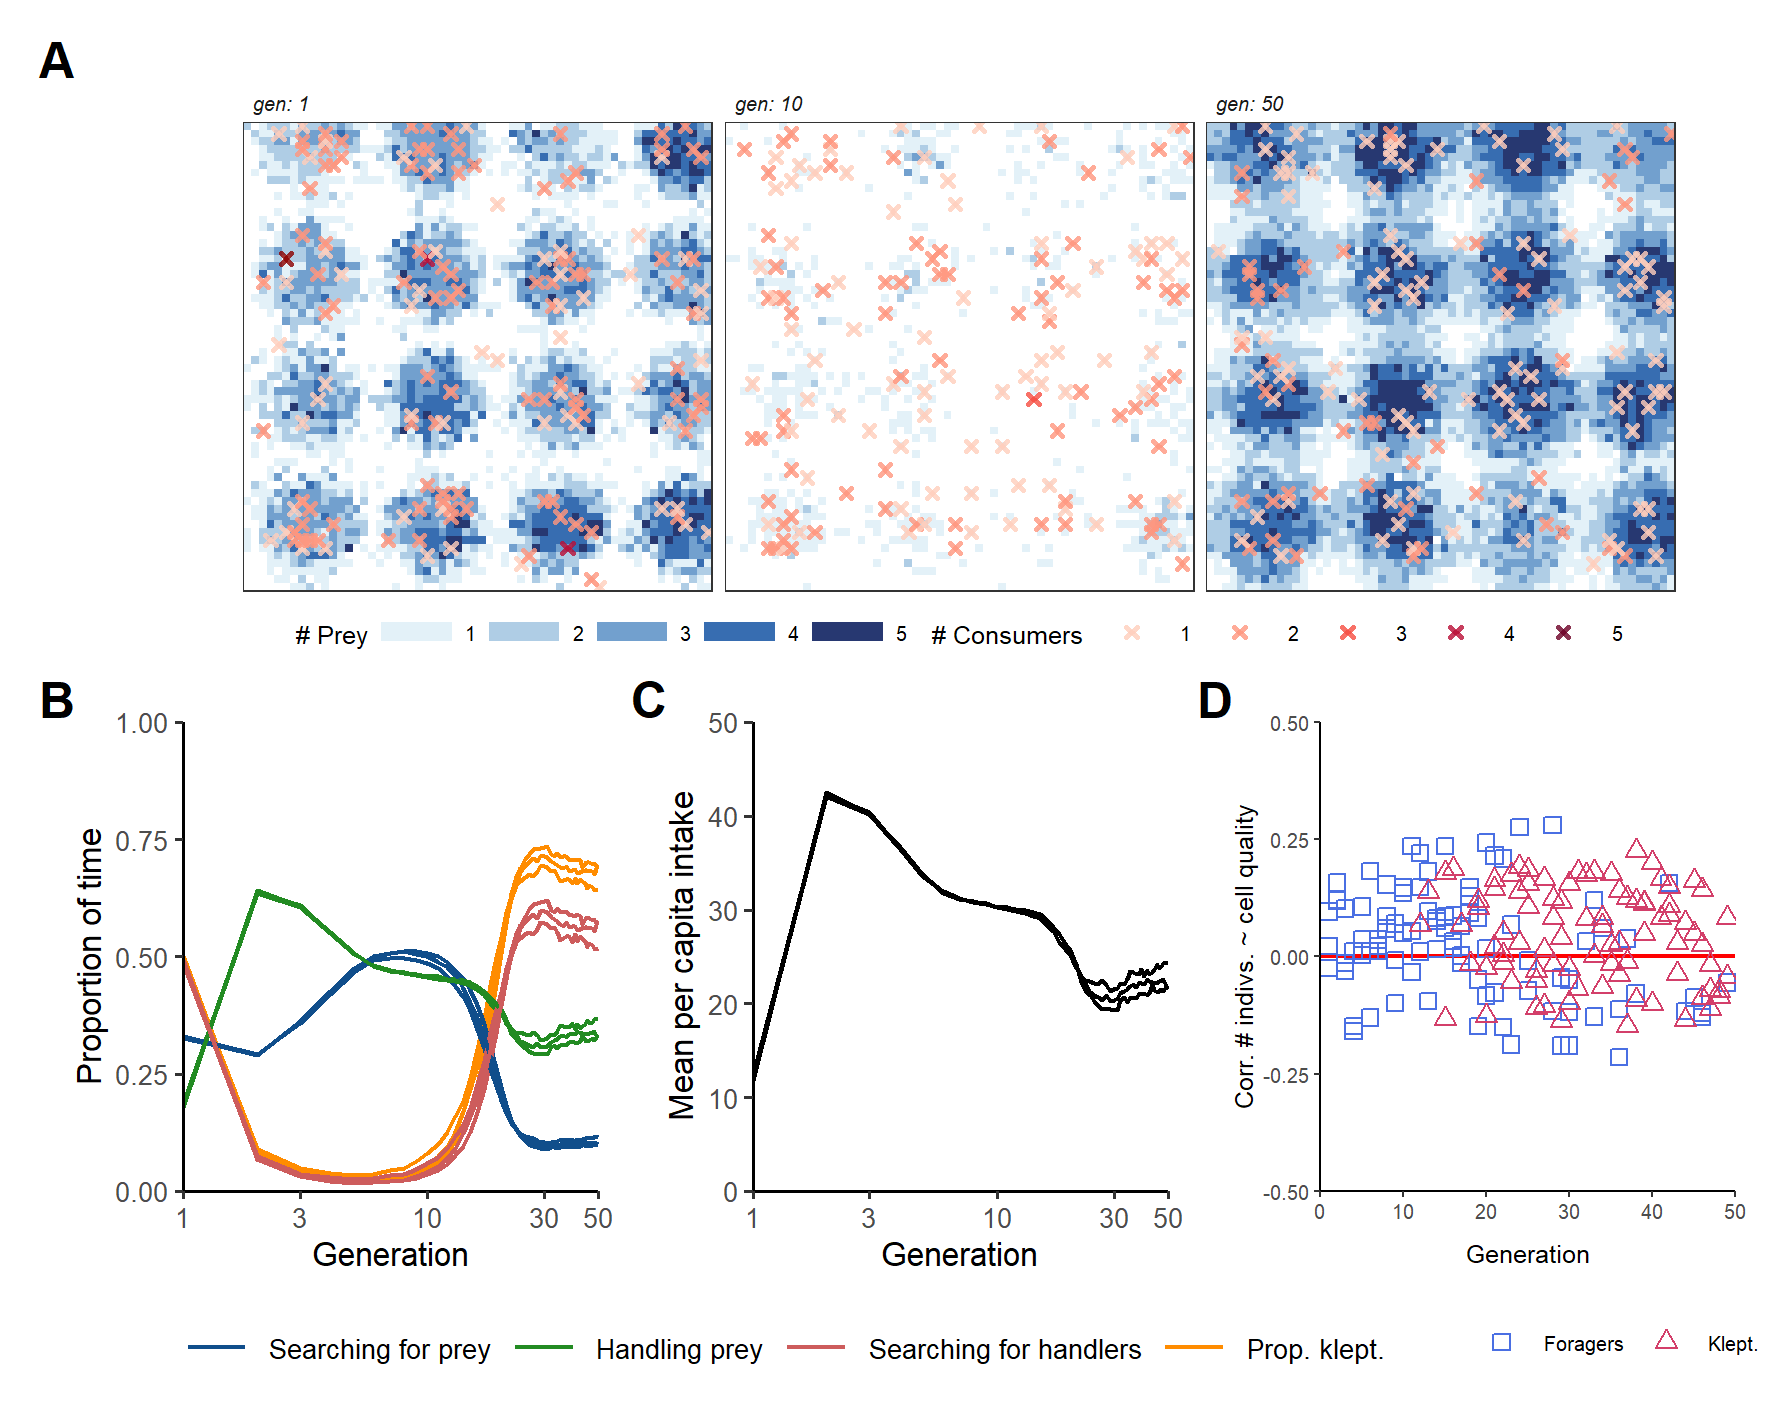
\includegraphics[width=0.70\textwidth]{figures/fig_02.png}
    \caption{
        \textbf{Eco-evolutionary implications of pure exploitation competition (Scenario 1).}
        Within 20 generations of evolution, the population reaches an equilibrium in \textbf{(A)} the relative proportion of time spent on searching prey and handling prey, and in \textbf{(B)} the total intake of the population.
        \textbf{(C)} The sustained extraction of prey-items results in a rapid depletion of the resource landscape within 10 generations. The number of individuals on occupied cells is shown as black circles (size = number of individuals).
        At equilibrium, cell occupancy (number of foragers per cell) is only weakly correlated with cell productivity $r$ \textbf{(D)}, while it is even negatively correlated with the number of food items in the cell \textbf{(E)}.
        Panels \textbf{A, B, D} and \textbf{E} show three replicates, while panel \textbf{C} shows a single replicate; all panels are for $r_{max}$ = 0.01.
    }
    \label{Fig:Model1}
\end{figure}

\begin{figure}[h!]
    \centering
    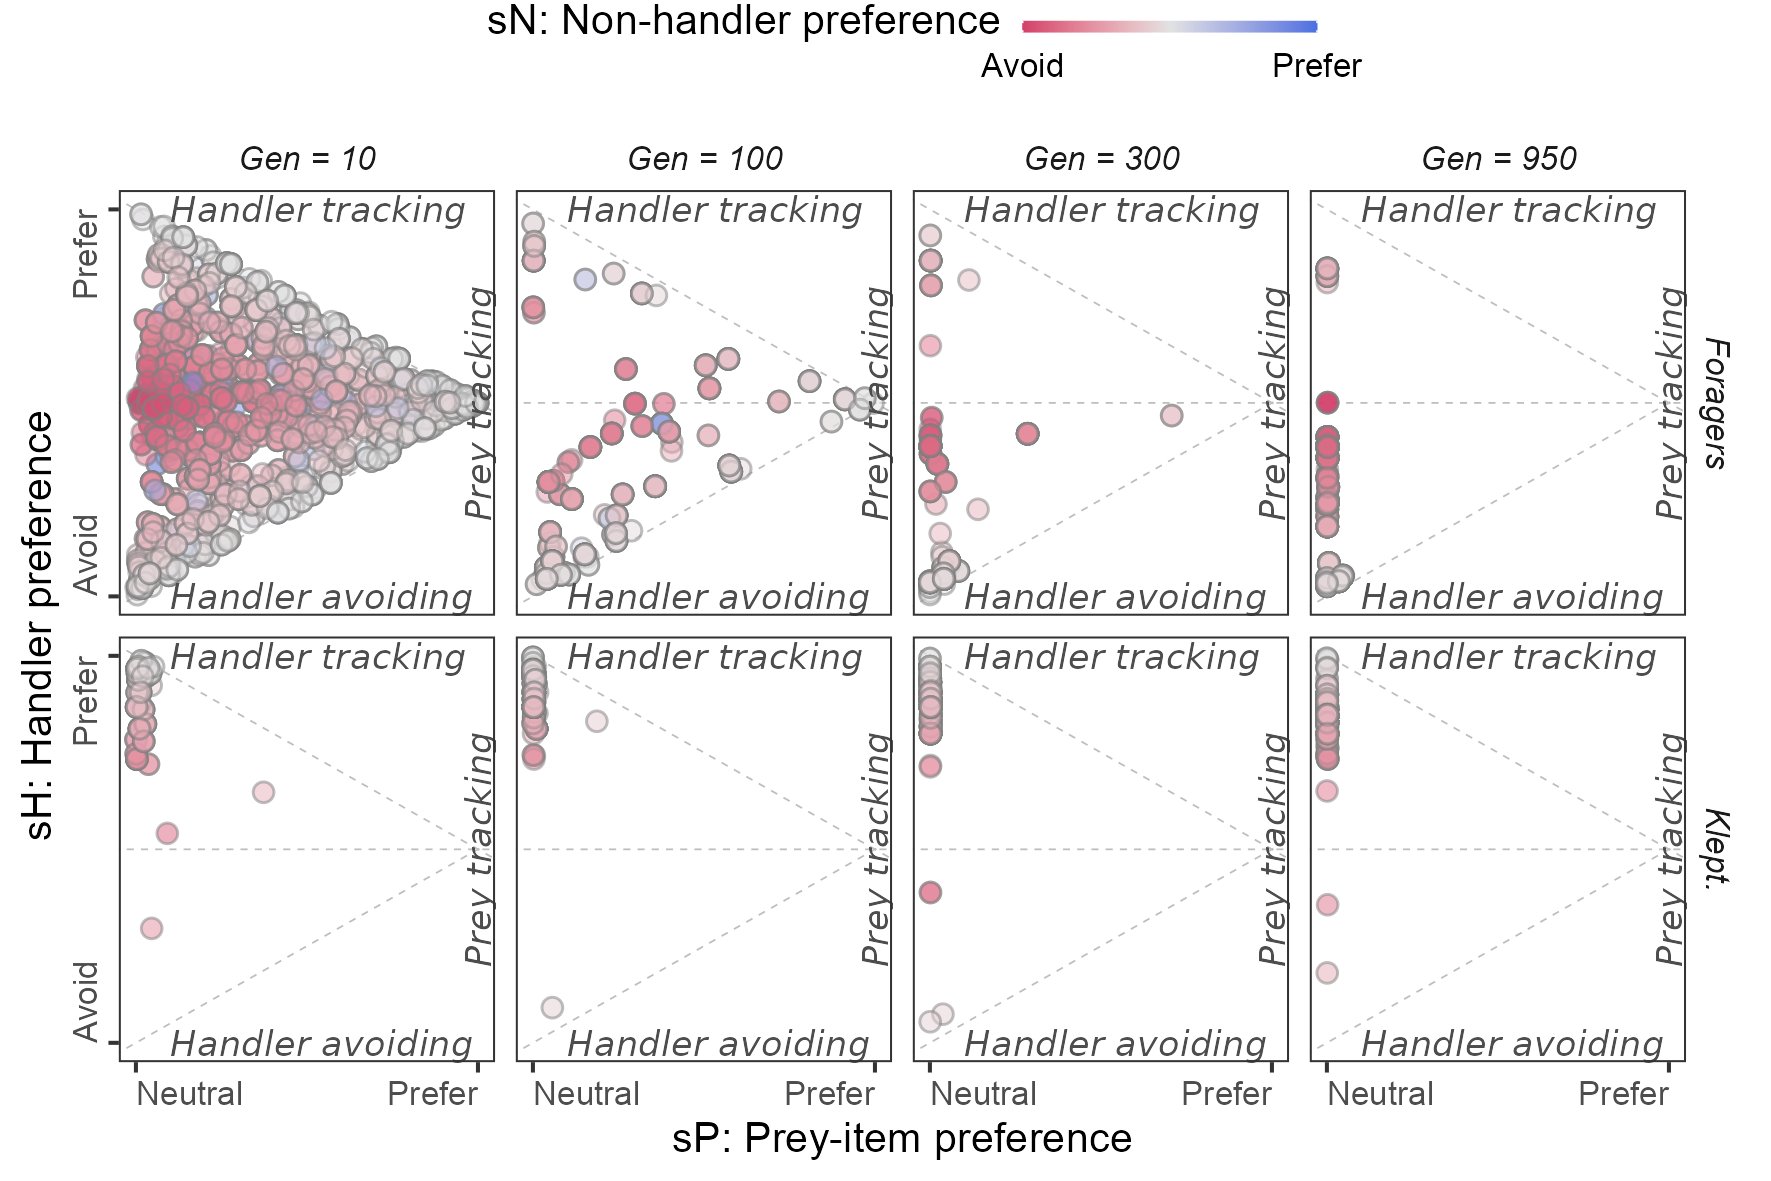
\includegraphics[width=0.70\textwidth]{figures/fig_03.png}
    \caption{
        \textbf{Eco-evolutionary implications of exploitation combined with a fixed foraging strategy (Scenario 2).}
        In Scenario 2, the population reaches an equilibrium in \textbf{(A)} the relative proportion of time spent on searching prey and handling prey, and in \textbf{(B)} the total intake of the population.
        Stealing activities (red line; panel A) are less common than kleptoparasitic individuals (orange line; panel A), as successful kleptoparasites become handlers (green line; panel A).
        \textbf{(C)} With a reduction in foraging and handling due to increased stealing after generation 30 (panel A), prey-item depletion is reduced, and the resource landscape recovers by generation 50.
        The number of individuals on occupied cells is shown as black circles (size = number of individuals). 
        At equilibrium, cell occupancy (number of foragers per cell) is only weakly correlated with cell productivity $r$ \textbf{(D)}, and weakly negatively correlated with the number of food items in the cell \textbf{(E)}.
        Panels \textbf{A, B, D} and \textbf{E} show three replicates, while panel \textbf{C} shows a single replicate; all panels are for $r_{max}$ = 0.01.
    }
    \label{Fig:Model2}
\end{figure}

\begin{figure}[h!]
    \centering
    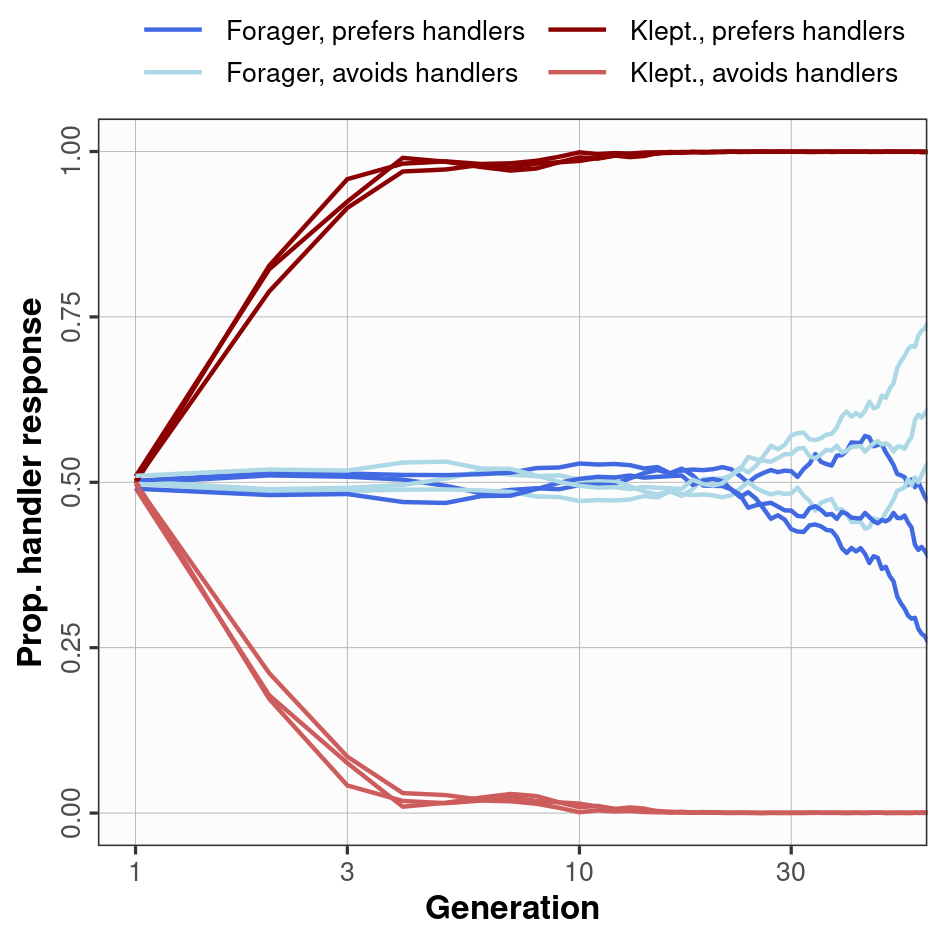
\includegraphics[width=0.70\textwidth]{figures/fig_07.png}
    \caption{
       \textbf{Rapid divergence of movement rules between fixed foraging strategies due to correlational selection (Scenario 2).}
       \textbf{(A)} Kleptoparasitism rapidly becomes the more frequent strategy in Model 2 populations, with no differences across replicates.
       \textbf{(B)} However, replicates differ strongly in the frequencies of evolved movement strategies among the two behavioural strategies.
       While nearly all kleptoparasites evolve to move towards handlers, their direct resource, the strength of their handler preference is polymorphic, with 2 or 3 morphs in most replicates.
       \textbf{(C)} Foragers are also polymorphic in their handler responses, but these morphs are the results of drift, rather than selection.
       \textbf{(D)} Overall, within 5 generations (shown on a log scale), all kleptoparasitic individuals ($\sim$75\% of the population at equilibrium; see Fig. 3A) have an evolved preference for moving towards handlers.
       Meanwhile, forager individuals are agnostic to handlers, and are equally split between handler preference and avoidance.
       All panels show three replicates at $r_{max}$ = 0.01.
    }
    \label{Fig:Syndrome}
\end{figure}

\begin{figure}[h!]
    \centering
    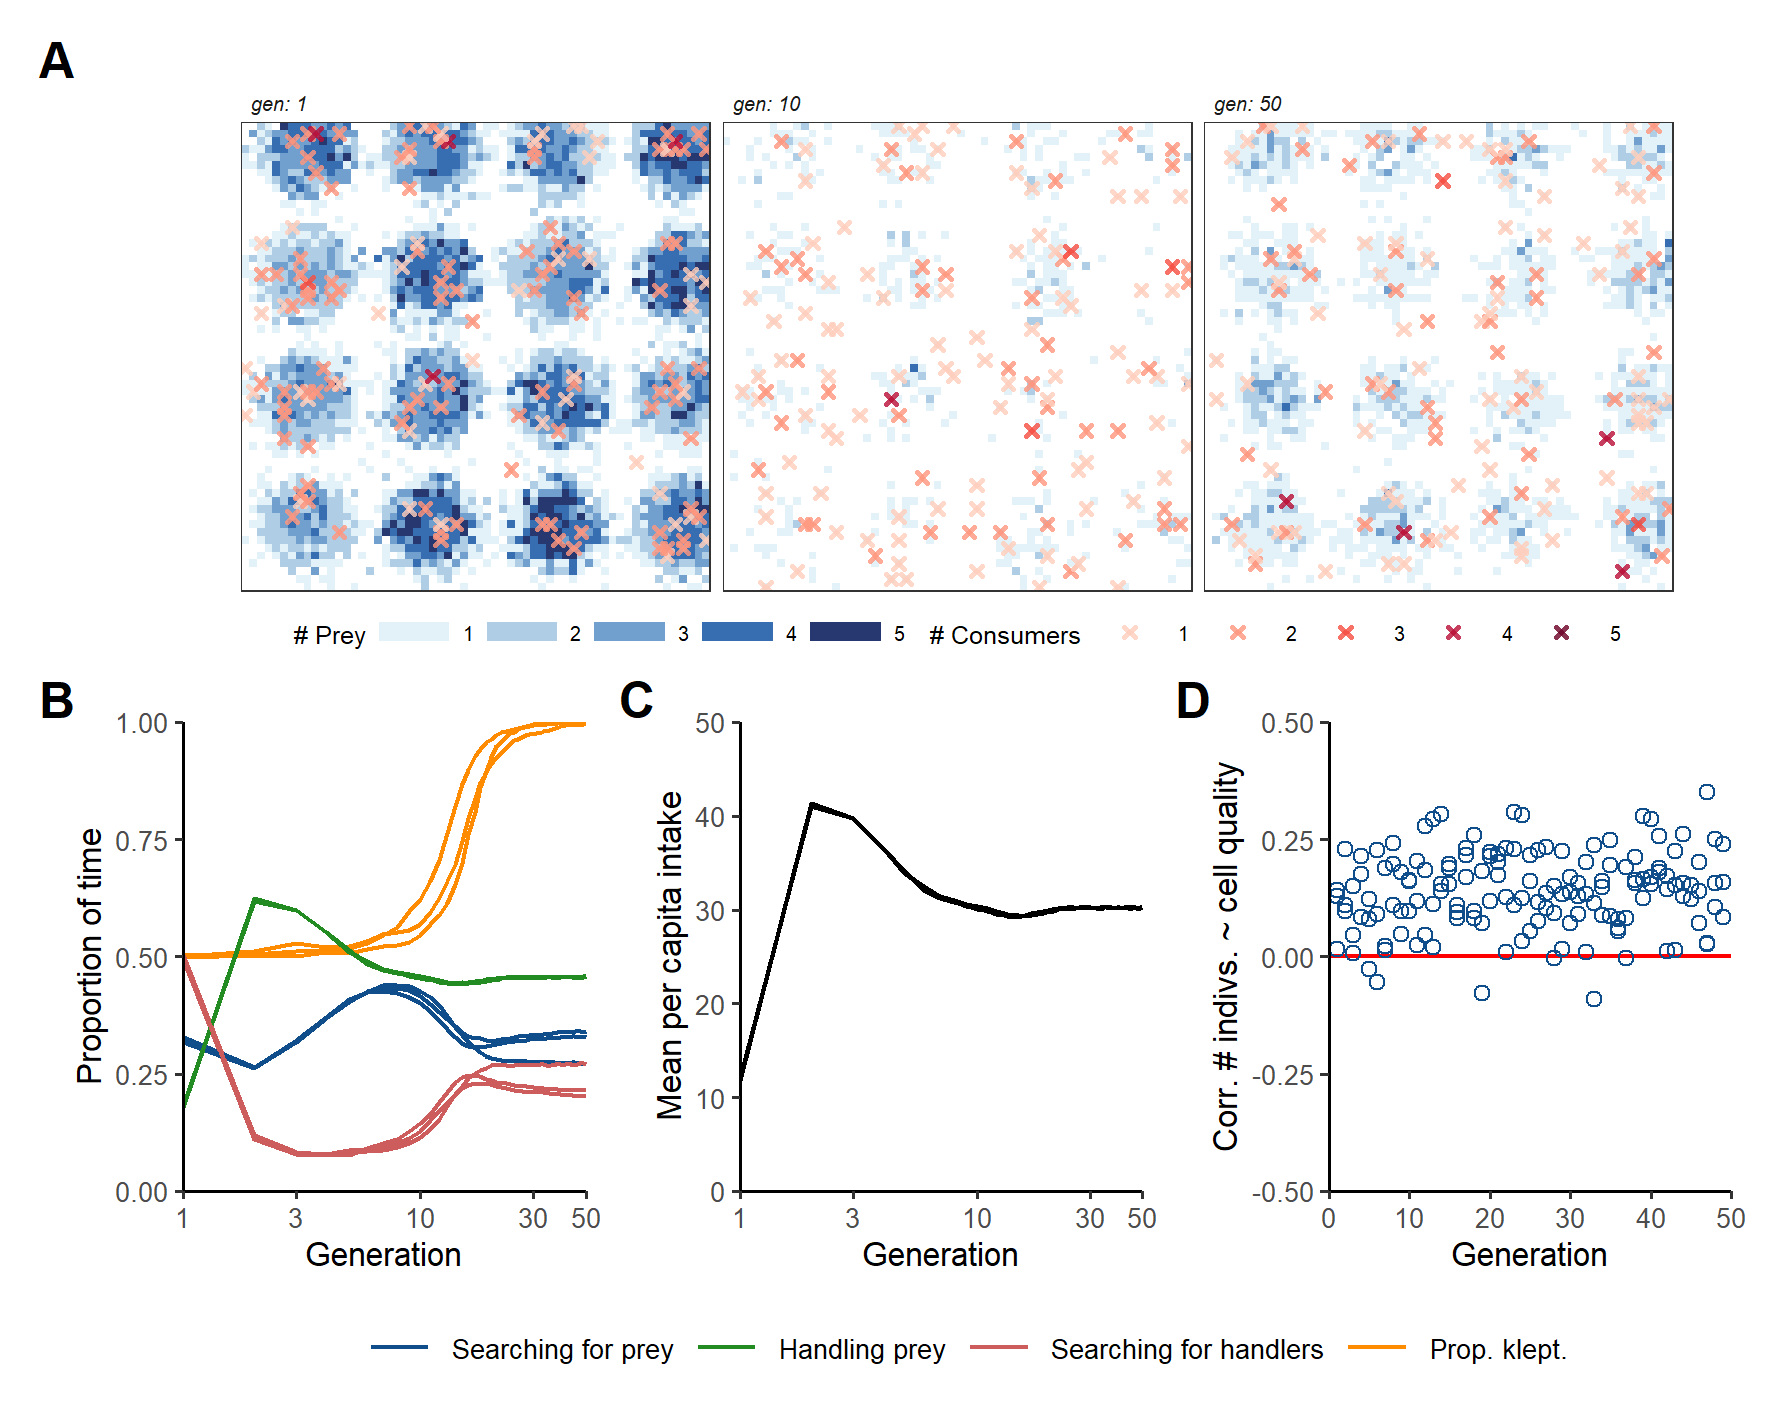
\includegraphics[width=0.70\textwidth]{figures/fig_04.png}
    \caption{
        \textbf{Eco-evolutionary implications of exploitation combined with a conditional foraging strategy (Scenario 3).}
        Scenario 3 populations reach an equilibrium in \textbf{(A)} the relative proportion of time spent on searching prey and handling prey, and in \textbf{(B)} the total intake of the population within 30 generations of evolution.
        While an opportunistic kleptoparasitic strategy (orange line; panel A) becomes rapidly fixed in the population, the actual frequency of stealing remains relatively much lower (red line; panel A).
        \textbf{(C)} The initially rapid depletion of the resource landscape within 10 generations is halted as kleptoparasitism reduces foraging activities, and the resource landscape regenerates prey-items by generation 50.
        The number of individuals on occupied cells is shown as black circles (size = number of individuals).
        \textbf{(D)} The correlation between the number of individuals on a cell, and its productivity $r_{max}$, and
        \textbf{(E)} the correlation between individual counts and the probability of finding a prey-item are both weak across generations.
        Panels \textbf{A, B, D} and \textbf{E} show three replicates, while panel \textbf{C} shows a single replicate; all panels are for $r_{max}$ = 0.01.
    }
    \label{Fig:Model3}
\end{figure}

\begin{figure}[h!]
    \centering
    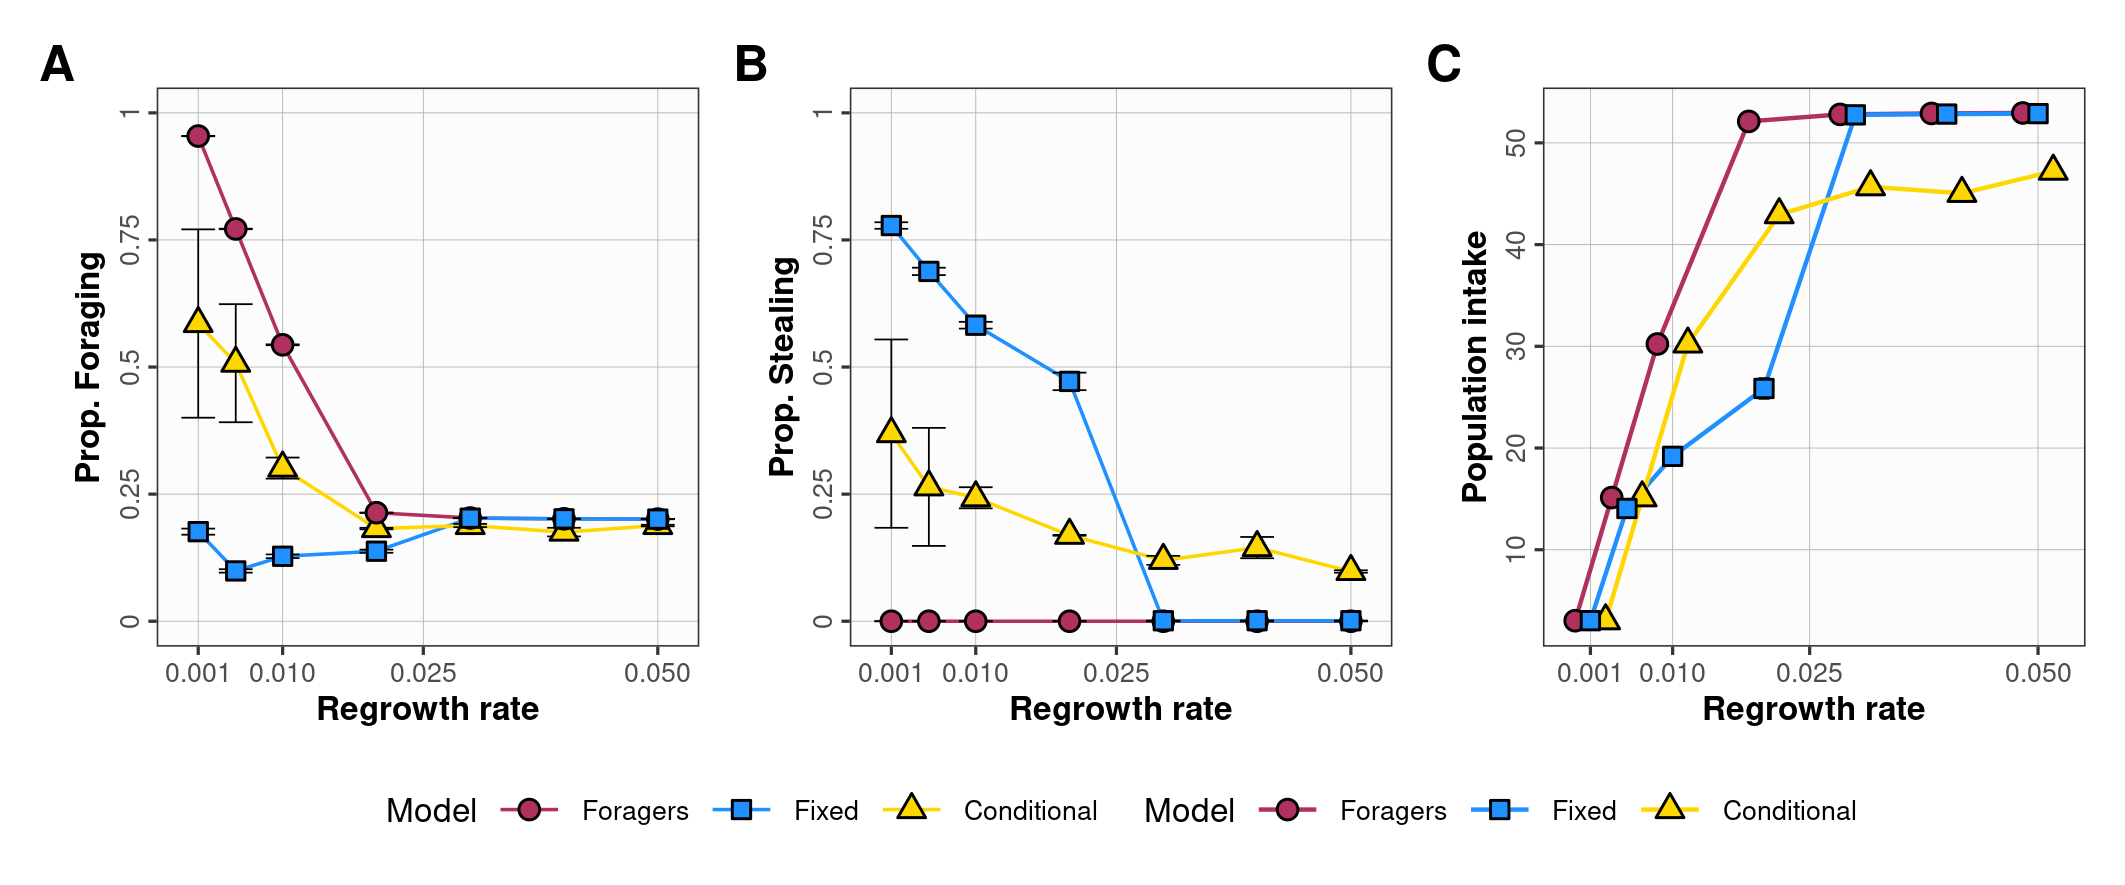
\includegraphics[width=0.85\textwidth]{figures/fig_06.png}
    \caption{Landscape productivity strongly affects model outcomes.
    \textbf{(A)} The frequency foraging reduces with increasing $r_{max}$ in models 1 and 3, but remains relatively stable in model 2. In all three models, this is partly due to an increase in handling caused by increased resoure availability, and \textbf{(B)} partly due to reduced kleptoparasitism in models 2 and 3. In model 2, kleptoparasitism goes extinct at higher $r_{max}$, and such model 2 populations are functionally identical with model 1 populations.
    \textbf{(C)} At low $r_{max}$, populations in all three models achieve similar intakes. At intermediate $r_{max}$ however, popualtions with a conditional kleptoparasitic strategy outperform populations with fixed strategies. At high $r_{max}$, conditional kleptoparasitism populations (model 3) achieve lower intakes than populations in models 1 and 2, which are then functionally identical.
    Shaded regions around solid lines show the standard deviation of each value; these are not visible when the standard deviaiton is very small.
    }
    \label{Fig:Sensitivity}
\end{figure}

\begin{figure}[h!]
    \centering
    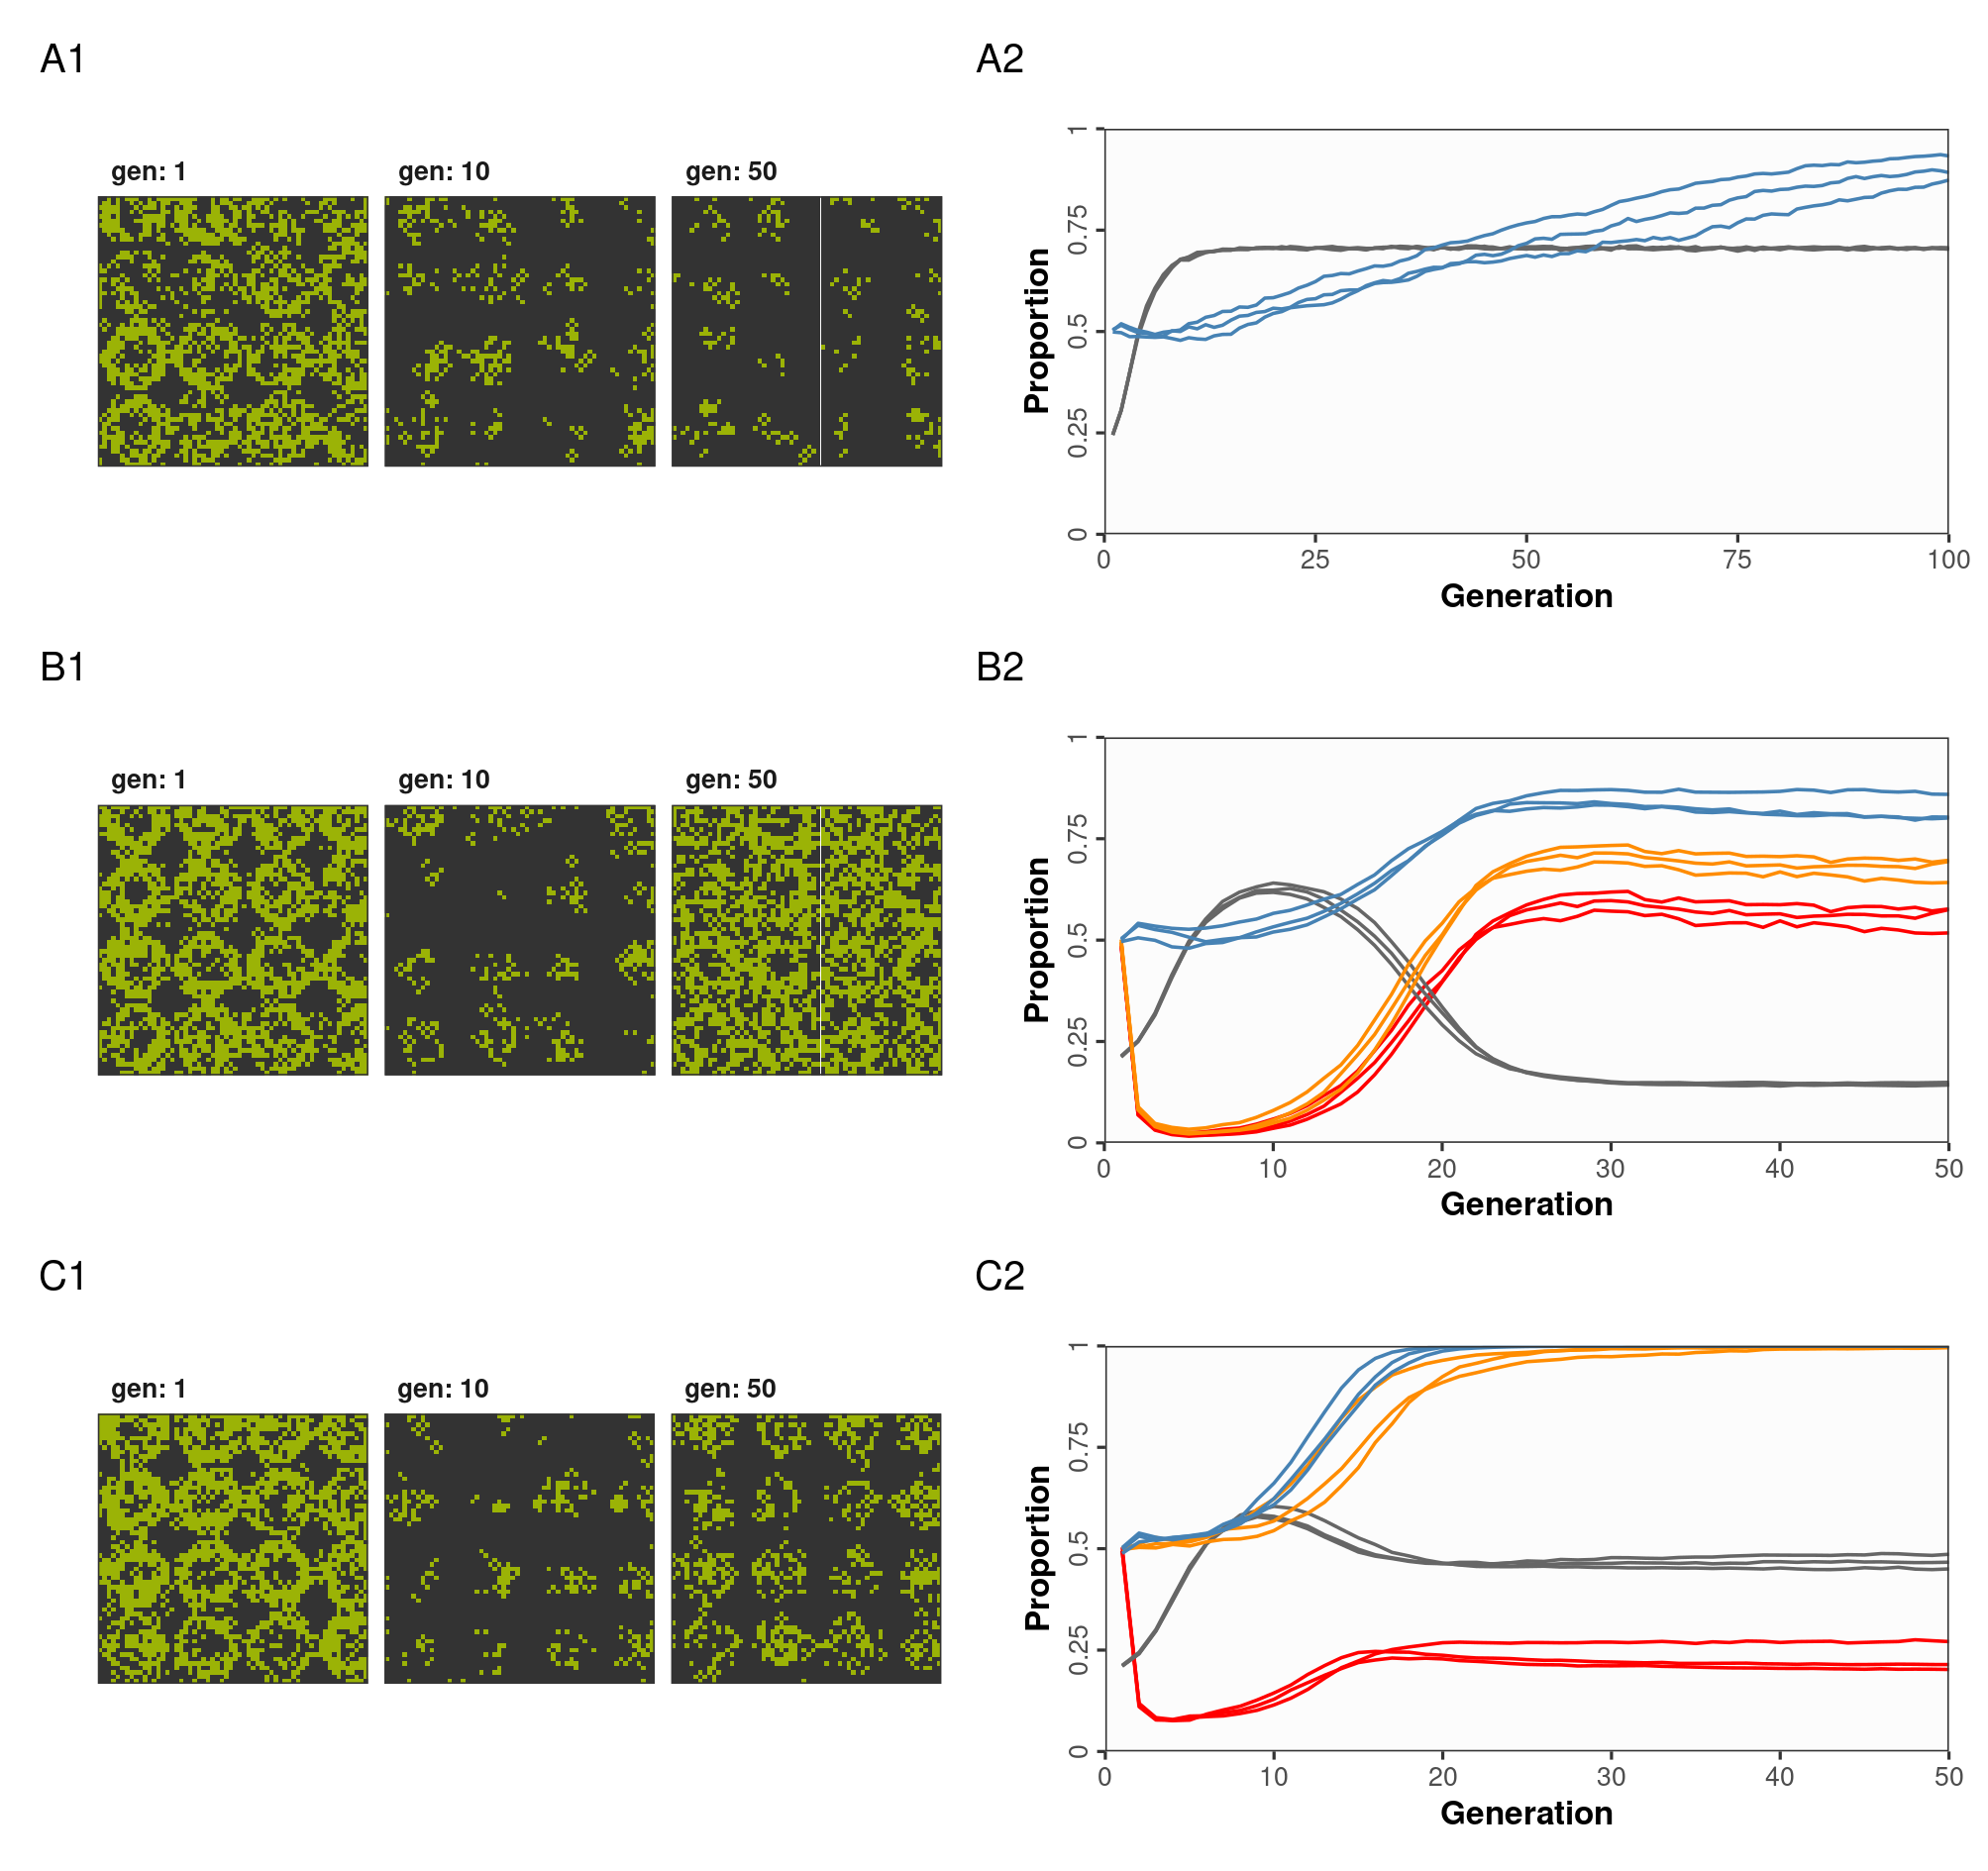
\includegraphics[width=0.70\textwidth]{figures/fig_08.png}
    \caption{
        The sustained depletion of prey-items leads to the homogenisation of large parts of the resource landscape within 10 generations.
        This homogenisation to zero items leads to the creation of `clueless regions', i.e., neighbouring cells with no difference in item counts, and thus no direct resource gradients (grey areas in \textbf{A1, B1, C1}; green areas show cells which differ from neighbours in item counts).
        Black lines in \textbf{(A2, B2, C2)} show the proportion of the landscape that is `clueless'.
        The evolution and persistence of a kleptoparasitic response (orange lines) and stealing events (red lines) reduces item depletion.
        \textbf{(A1, A2)} Strong depletion of the resource landscape in Model 1 leads to large areas with no item gradient.
        When the majority of the landscape is `clueless', moving towards handlers, which are an indirect indicator of resources, becomes a common strategy (blue line).
        \textbf{(B1, B2)} The emergence and persistence of fixed kleptoparasitism in Model 2 leads to a reduction in the area of clueless plateaus within 40 generations.
        \textbf{(C1, C2)} In Model 3, the conditional kleptoparasitic strategy leads to depletion intermediate between Models 1 and 2, and a similarly intermediate proportion of clueless plateaus on the landscape.
        All panels show replicates at $r_{max}$ = 0.01; landscape panels show only a single replicate.
    }
    \label{Fig:CluelessLandscape}
\end{figure}



% \subsection{Online figure legends}

% \renewcommand{\thefigure}{A\arabic{figure}}
% \setcounter{figure}{0}

% % \begin{figure}[h!]
% % %\includegraphics{jumps20m}
% % \caption{\textit{A}, the quick red fox proceeding to jump 20~m straight into the air over not one, but several lazy dogs. \textit{B}, the quick red fox landing gracefully despite the skepticism of naysayers.}
% % \label{Fig:Jumps}
% % \end{figure}

% % \begin{figure}[h!]
% % %\includegraphics{jumps20m}
% % \caption{The quicker the red fox jumps, the likelier it is to land near an okapi. For further details, see \citet{LemKapEx07}.}
% % \label{Fig:JumpsOk}
% % \end{figure}

% \renewcommand{\thefigure}{B\arabic{figure}}
% \setcounter{figure}{0}

\end{document}
